%%%%%%%%%%%%%%%%%%%%%%%%%%%%%%%%%%%%%%%%%%%%%%%%%%%%%%%%%%%%%%%%%%%%%%%%%%%%%
%% Documento base para criação de apresentações do LabEPI.                 %%
%% Aluno: Nome do Aluno <aluno@labepi.ufrn.br>                             %%
%% Orientador: Nome do Orientador <orientador@labepi.ufrn.br>              %%
%%%%%%%%%%%%%%%%%%%%%%%%%%%%%%%%%%%%%%%%%%%%%%%%%%%%%%%%%%%%%%%%%%%%%%%%%%%%%

\documentclass[10pt]{beamer}

\usepackage{beamerthemelabepi}
%\usepackage[T1]{fontenc}
\usepackage[latin1]{inputenc}
\usepackage{amsmath,amsthm,amssymb}
\usepackage[portuges,brazil]{babel}
\usepackage{booktabs}
\usepackage{thmtools}
\usepackage{lmodern}

%%%%%%%%%%%%%%%%%%%%%%%%%%%%%%%%%%%%%%%%%%%%%%%%%%%%%%%%%%%%%%%%%%%%%%%%%%%%%

\usecolortheme{labepi}
\setbeamertemplate{navigation symbols}{}
\addtobeamertemplate{navigation symbols}{}{\insertframenumber}

\newcommand\fontvii{\fontsize{8}{7.2}\selectfont}

\declaretheoremstyle[qed=$\square$]{thmsty}
\declaretheorem[style=thmsty,name=Teorema]{teorema}
\declaretheorem[style=thmsty,name=Corolário]{corolario}

%%%%%%%%%%%%%%%%%%%%%%%%%%%%%%%%%%%%%%%%%%%%%%%%%%%%%%%%%%%%%%%%%%%%%%%%%%%%%

\title{Modelo para Criação de Apresentações do LabEPI}
\subtitle{\normalfont Para defesas de TCC e Apresentações de Trabalhos}

\author{Nome Completo do Aluno ou Autor(es)}

\institute{%
% Para defesas de TCC usar as quatro linhas abaixo
Orientador: Prof. Dr. Nome Completo do Orientador\\
\vspace{0.1in}
(Defesa de Trabalho de Conclusão de Curso)
\vspace{0.1in}

\parbox{0.3\textwidth}{%
\centering
\includegraphics[width=0.25\textwidth]{image/ufrn.eps}}%
\parbox{0.55\textwidth}{%
\begin{center}%
Universidade Federal do Rio Grande do Norte -- UFRN\\
Centro de Ensino Superior do Seridó -- CERES\\
Departamento de Computação e Tecnologia -- DCT\\
Bacharelado em Sistemas de Informação -- BSI
\end{center}}

\vspace{0.1in}

\includegraphics[width=0.15\textwidth]{image/labepi}\hspace{0.1in}\\
Laboratório de Elementos do Processamento da Informação -- LabEPI}

\date{\small\today}

%%%%%%%%%%%%%%%%%%%%%%%%%%%%%%%%%%%%%%%%%%%%%%%%%%%%%%%%%%%%%%%%%%%%%%%%%%%%%
\begin{document}

\frame{\titlepage}

% ------------------------------------------------------------------------- %
\begin{frame}
    \frametitle{Problema}

Projeto de Sistemas de Monitoramento de Redes de Computadores

\vfill

\centering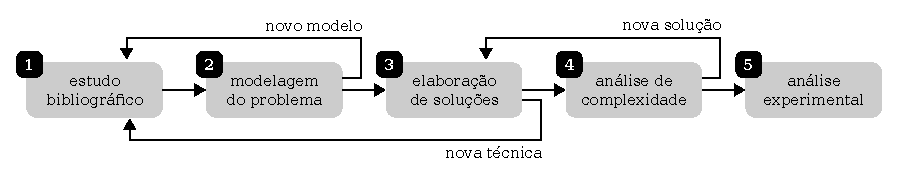
\includegraphics[scale=0.73]{image/metodologia}

\end{frame}

% ------------------------------------------------------------------------- %
\begin{frame}
    \frametitle{Trabalhos relacionados}

\begin{minipage}{0.55\textwidth}
{\bf Observabilidade}\small
\begin{itemize}
\item Cáceres et al. (1999)
    \begin{itemize}
    \item modelo {\it multicast}
    \end{itemize}
\item Ji \& Elwalid (2002)
    \begin{itemize}
    \item escalabilidade da quantidade de medições
    \end{itemize}
\item Chen et al. (2007)
    \begin{itemize}
    \item quantidade de nós monitores da ordem de $O(n \log n)$,
        monitoramento de {\it links}
    \end{itemize}
\item Gopalan \& Ramasubramanian (2012)
    \begin{itemize}
    \item localização dos nós observadores
    \end{itemize}
\end{itemize}
\end{minipage}%
\begin{minipage}{0.45\textwidth}
{\bf Visualização}\small
\begin{itemize}
\item Yee et al. (2001)
    \begin{itemize}
    \item visualização radial interativa
    \end{itemize}
\item Bachmaier (2007)
    \begin{itemize}
    \item planaridade radial
    \end{itemize}
\item Diehl et al. (2010)
    \begin{itemize}
    \item tempo de resposta similares
    \end{itemize}
\item Burch et al. (2011)
    \begin{itemize}
    \item tempo de resposta no centro da visualização
    \end{itemize}
\end{itemize}
\end{minipage}

\end{frame}

% ------------------------------------------------------------------------- %
\begin{frame}
    \frametitle{Proposta}

\begin{block}{O problema da escolha dos observadores}
Dado que a topologia da rede é conhecida, como escolher de forma ótima,
dentre os nós acessíveis na topologia, aqueles que desempenharão o papel de
observadores?
\end{block}

\vfill

Utilização da teoria de representação de redes como sistemas lineares para
explorar o conceito de observabilidade.

\end{frame}

% ------------------------------------------------------------------------- %
\begin{frame}
    \frametitle{Proposta}

\begin{block}{O problema da apresentação da informação}
Dado um conjunto de predicados, como é possível apresenta-los de forma
eficiente, escalável e eficaz, considerando a utilização do fator visual e da
ampliação da cognição que ela proporciona?
\end{block}

\vfill

Minimização do tempo e da quantidade de recursos necessários para
apresentação dos predicados por meio da visualização por disposição radial.

\end{frame}

% ------------------------------------------------------------------------- %
\begin{frame}
    \frametitle{Organização}

\begin{itemize}
\item Observabilidade
    \begin{itemize}
    \item Conceitos: estrutural e funcional
    \item Premissas
    \item Modelo
    \item Resultados teóricos
    \item Experimentos
    \end{itemize}
\item Visualização
    \begin{itemize}
    \item Conceitos
    \item Premissas
    \item Modelo
    \item Resultados teóricos
    \item Experimentos
    \end{itemize}
\item Considerações finais
\end{itemize}

\end{frame}

% ------------------------------------------------------------------------- %
\begin{frame}
    \frametitle{Observabilidade}

\begin{block}{Observabilidade estrutural}
Conjunto de nós para os quais a leitura dos estados permitem a inferência do
estado de todos os outros nós da rede.
\end{block}

\vfill

\begin{block}{Observabilidade funcional}
Conjunto de nós cuja quantidade de informação que trafega por eles consiste
em um fator predefinido da totalidade do tráfego que se propaga na rede.
\end{block}

\vfill

Busca-se a minimização desses conjuntos para atender os requisitos de
escalabilidade.
\end{frame}

% ------------------------------------------------------------------------- %
\begin{frame}
    \frametitle{Observabilidade estrutural}

\begin{block}{Invariância topológica}
Considera-se que a topologia da rede não muda com o tempo.
Essa propriedade é denominada invariância topológica restrita.
\end{block}

\vfill

\begin{block}{Evolução discreta de estado}
A transição de estado do sistema ocorre de forma síncrona, para cada nó da
rede, e discreta, em instantes bem definidos.
\end{block}

\end{frame}

% ------------------------------------------------------------------------- %
\begin{frame}
    \frametitle{Observabilidade funcional}

\begin{block}{Conservação da informação}
A probabilidade de haver perda de informação na rede durante o processo de
propagação é nula.
\end{block}

\vfill

\begin{block}{Atingibilidade}
A probabilidade de que uma informação partindo de um nó qualquer da rede
atinja qualquer outro nó da rede é sempre positiva.
\end{block}

\end{frame}

% ------------------------------------------------------------------------- %
\begin{frame}
    \frametitle{Observabilidade funcional}

\begin{block}{Processo markoviano}
Um processo de Markov é uma descrição de um sistema cujo estado
$\mathbf{x}(t)$ evolui da seguinte forma:
\begin{equation*}
    \mathbf{x}(t+1) = \mathbf{P} \mathbf{x}(t)\text{,}
\end{equation*}
onde $\mathbf{P}$ é uma matriz estocástica de transição de estado definida
como
\begin{equation*}
\mathbf{P} =
\begin{bmatrix}
    p_{11} & \dotsb & p_{1n} \\
    \vdots & \ddots & \vdots \\
    p_{n1} & \dotsb & p_{nn} 
\end{bmatrix}\text{,}
\end{equation*}
onde $p_{ij}$ descreve a probabilidade de ocorrência no estado $x_i(t+1)$
dada uma ocorrência precedente em $x_j(t)$.
\end{block}

\end{frame}

% ------------------------------------------------------------------------- %
\begin{frame}
    \frametitle{Visualização}

\begin{teorema}[Tempo de execução esperado do algoritmo]
O tempo esperado de execução necessário para se calcular o raio base mínimo
para visualização por disposição radial expressiva é da ordem de $\Theta(n)$,
ou seja, linear e proporcional a quantidade de nós.
\end{teorema}

\vfill

\begin{teorema}[Escalabilidade da visualização]
A quantidade de nós $n$ em uma visualização por disposição radial expressiva
mínima com área $A$ é dada pela relação assintótica $n\in\Theta(A^\alpha)$,
onde $1/2 \leq \alpha \leq 1$.
Sendo que, para $\alpha=1/2$, caracteriza-se o pior caso de escalabilidade, e
para $\alpha=1$, o melhor caso.
\end{teorema}

\end{frame}

% ------------------------------------------------------------------------- %
\begin{frame}
    \frametitle{Conclusões}

{\bf Observabilidade}

\footnotesize
\begin{tabular}{lcc}
\toprule
métrica     & observabilidade estrutural $|O^o_e|$
            & observabilidade funcional  $|O^o_c|$ \\
\midrule
densidade   & inversa  
            & direta  \\
grau médio  & inferior
            & superior\\
diâmetro    & inversa 
            & direta  \\
eficiência  & direta  
            & inversa \\
agrupamento & direta  
            & inversa \\
\bottomrule
\end{tabular}

\vfill

\normalsize
{\bf Visualização}

\footnotesize
\begin{tabular}{p{7em}cc}
\toprule
métrica     & raio total para $m=1$ & raio total para $m=2$ \\
\midrule
diâmetro    & direta & invariante \\
eficiência  & direta & direta \\
\bottomrule
\end{tabular}

\end{frame}

% ------------------------------------------------------------------------- %
\begin{frame}
    \frametitle{Contribuições}

{\bf Observabilidade}

\begin{itemize}
\item Demonstração da possíbilidade de inferência do estade da rede a partir
    do monitoramento de um subconjunto de nós;
\item Algoritmos de tempo linear para definição dos conjuntos observadores
    mínimos;
\item Observações com base em experimentos que relacionam métricas da rede
    com a quantidade mínima de nós observadores;
\end{itemize}

{\bf Visualização}

\begin{itemize}
\item Minimização do espaço necessário para representação expressiva pela
    disposição radial;
\item Algoritmo de tempo linear para otimização da visualização;
\item Demonstração dos limites teóricos de escalabilidade;
\item Observações com base em experimentos que relacionam métricas da rede
    com a escalabilidade da visualização.
\end{itemize}

\end{frame}

% ------------------------------------------------------------------------- %
\begin{frame}
    \frametitle{Produção}\fontvii

{\bf Capítulos de livros}

\begin{itemize}
\item Medeiros, J.P.S.; Borges Neto, J.B.; Brito Júnior, A.M.; Pires, P.S.M.
    {\bf Learning Remote Computer Fingerprinting},
    Computational Intelligence in Digital Forensics, Springer, Intelligent
    Systems Reference Library, ISSN 1868-4394, 2014 (aceito para publicação).
\item Medeiros, J.P.S.; Borges Neto, J.B.; Queiroz, G.S.D.; Pires, P.S.M.
    {\bf Intelligent Remote Operating System Detection}, Case Studies in
    Secure Computing, Achievements and Trends, CRC Press, Taylor and Francis,
    2014 (aceito para publicação).
\end{itemize}

{\bf Periódicos}

\begin{itemize}
\item Medeiros, J.P.S.; Santos, S.R.; Brito Júnior, A.M.; Pires, P.S.M.
    {\bf Advances in Network Topology Security Visualisation}, International
    Journal of System of Systems Engineering (IJSSE), ISSN 1748-0671,
    Inderscience, volume 1, number 4, pages 387-400, 2009.
\item Medeiros, J.P.S.; Brito Júnior, A.M.; Pires, P.S.M.
    {\bf Using Intelligent Techniques to Extend the Applicability of
    Operating System Fingerprint Databases}, Journal of Information Assurance
    and Security (JIAS), ISSN 1554-1010, volume 5, issue 4, pages 554-560,
    2010.
\item Medeiros, J.P.S.; Pires, P.S.M.
    {\bf On the Scalability Bounds of Radial Layout for the Visualization of
    Scale-free Networks},
    Applicable Algebra in Engineering, Communication and Computing (AAECC),
    ISSN 0938-1279, Springer, 2013 (submetido para revisão).
\end{itemize}

\end{frame}

% ------------------------------------------------------------------------- %
\begin{frame}
    \frametitle{Produção}\fontvii

{\bf Conferências}

\begin{itemize}
\item Medeiros, J.P.S.; Brito Júnior, A.M.; Pires, P.S.M.
    {\bf A New Method for Recognizing Operating Systems of Automation
    Devices},
    14th IEEE International Conference on Emerging Technologies and Factory
    Automation (ETFA), 2009.
    Proceedings of ETFA 2009, ISSN 1946-0759, pages 1-4,
    ISBN 978-1-4244-2727-7, 2009.
\item Medeiros, J.P.S.; Brito Júnior, A.M.; Pires, P.S.M.
    {\bf A Data Mining Based Analysis of Nmap Operating System Fingerprint
    Database},
    2nd International Workshop on Computational Intelligence in Security for
    Information Systems (CISIS), 2009.
    Advances in Soft Computing, ISSN 1867-5662, volume 63, pages 1-8,
    Springer, 2009.
\item Medeiros, J.P.S.; Brito Júnior, A.M.; Pires, P.S.M.
    {\bf An Effective TCP/IP Fingerprinting Technique Based on Strange
    Attractors Classification},
    2nd International Workshop on Autonomous and Spontaneous Security
    (SETOP), 2009.
    Lecture Notes in Computer Science (LNCS), ISSN 0302-9743, volume 5939,
    pages 208-221, Springer, 2010.
\item Medeiros, J.P.S.; Brito Júnior, A.M.; Pires, P.S.M.
    {\bf A Qualitative Survey of Active TCP/IP Fingerprinting Tools and
    Techniques for Operating Systems Identification},
    4th International Workshop on Computational Intelligence in Security for
    Information Systems (CISIS), 2011.
    Lecture Notes in Computer Science (LNCS), ISSN 0302-9743, volume 6694,
    pages 68-75, Springer, 2011.
\item Medeiros, J.P.S.; Pires, P.S.M.
    {\bf Optimal Visualization of Complex Networks Using Radial Layout},
    Perspectives and Challenges in Statistical Physics and Complex Systems
    for the Next Decade: A Conference in Honor of Eugene Stanley and Liacir
    Lucena, Book of Abstracts, page 37, 2011.
\end{itemize}

\end{frame}

% ------------------------------------------------------------------------- %
\begin{frame}
    \frametitle{Trabalhos futuros}

{\bf Observabilidade}

\begin{itemize}
\item Estudo da validade do modelo considerando premissas menos restritivas;
\item Projetar um sistema de monitoramento como prova de conceito;
\item Estudar mecanismos de ajuste da matriz de transição de estrados para o
    caso variante no tempo;
\item Estudar projeto de topologias menos sucetíveis à ataques distriuídos.
\end{itemize}

\vfill

{\bf Visualização}

\begin{itemize}
\item Extensão do modelo para utilização de técnicas de distorção;
\item Verificar demais propriedades da rede relacionadas à escalabilidade.
\end{itemize}

\end{frame}

\end{document}
%%%%%%%%%%%%%%%%%%%%%%%%%%%%%%%%%%%%%%%%%%%%%%%%%%%%%%%%%%%%%%%%%%%%%%%%%%%%%
%%%%%%%%%%%%%%%%%%%%%%%%%%%%%%%%%%%%%%%%%%%%%%%%%%%%%%%%%%%%%%%%%%%%%%%%%%%%%
